\documentclass[12pt,a4paper]{article}
\usepackage{amsmath}
\usepackage{mathtext}
\usepackage{icomma}
\usepackage{amsfonts}
\usepackage{amssymb}
\usepackage[utf8]{inputenc}
\usepackage[T1,T2A]{fontenc}
\usepackage[english, russian]{babel}
\usepackage{graphicx}
\usepackage[left=2cm,right=2cm,top=2cm,bottom=2cm]{geometry}
\usepackage{calc}
\usepackage{wrapfig}
\usepackage{setspace}
\usepackage{indentfirst}
\usepackage{subfigure}
\usepackage[table,xcdraw]{xcolor}


\title{
Отчет о выполнении лабораторной работы 3.3.4 \\
Эффект Холла в полупорводниках}
\author{Исламов Сардор, группа Б02-111}
% \date{}

\begin{document}

\maketitle

\subparagraph*{Аннотация.} 
В данной работе проведено измерение подвижности и концентрации носителей заряда в полупроводниках посредством изучения зависимости ЭДС Холла от внешнего магнитного поля и тока, протекающего по образцу.
Также определен тип проводимости образца. 

\subsection*{Теоретическое введение}
Пусть через однородную пластину металла вдоль оси $x$ течет ток $I$ (рис. 1).
	
	\begin{wrapfigure}{l}{0.6\textwidth}
		\vspace{-20pt}
		\begin{center}
			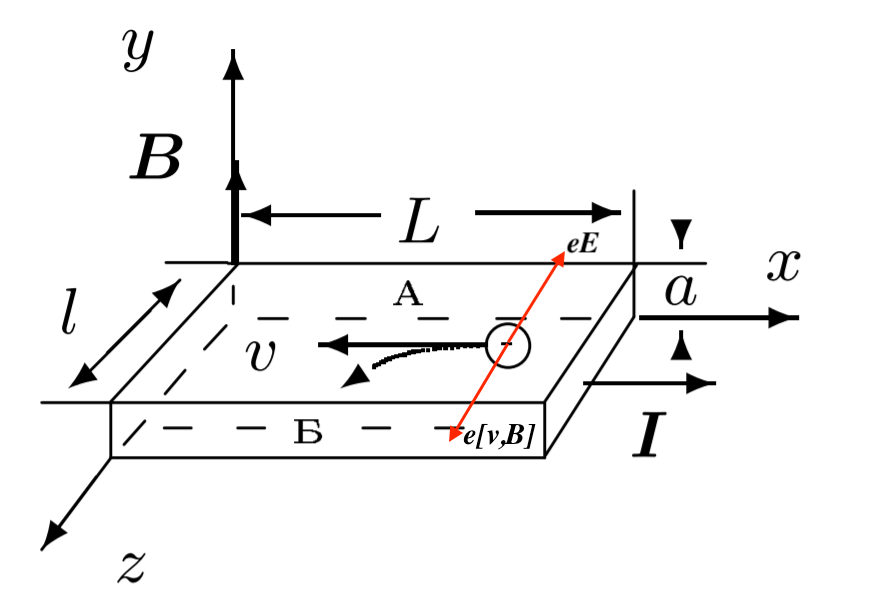
\includegraphics[width=0.7\linewidth]{Holl1.png}
			\label{fig:sdfsafd}
		\end{center}
		\vspace{-20pt}
		\caption{Образец с током в магнитном поле}
	\end{wrapfigure}

	Если эту пластину поместить в магнитное поле, направленное по оси y, то между гранями А и Б появляется разность потенциалов. 
	
	В самом деле, на электрон (для простоты рассматриваем один тип носителей), движущийся со средней скоростью $\langle \vec{v} \rangle$ в электромагнитном поле, действует сила Лоренца:
	
	$$\vec{F}_{л} = -e\vec{E}-e \langle \vec{v} \rangle \times \vec{B},$$
	
	где $e$- абсолютный заряд электрона, $\vec{E}$ - напряженность электрического поля, $\vec{B}$ - индукция магнитного поля.
	
	В проекции на ось $z$ получаем
	
	$$ F_{B}=e | \langle {v_{x}} \rangle | B.$$
	
	Под действием этой силы электроны отклоняются к грани Б, заряжая ее отрицательно. На грани А накапливаются нескомпенсированные положительные заряды. Это приводит к возникновению электрического поля $E_{z}$, направленного от А к Б, которое действует на электроны с силой $F_{E}=eE_{z}$. В установившемся режиме $F_{E}=F_{B}$, поэтому накопление электрических зарядов на боковых гранях пластины прекращается. Отсюда
	
	$$ E_{z}=| \langle {v_{x}} \rangle | B.$$
	
	С этим полем связана разность потенциалов $$U_{AБ}=E_{z}l=| \langle {v_{x}} \rangle | Bl.$$
	
	В этом и состоит эффект Холла.
	
	\
	
	Замечая, что сила тока $ I=ne| \langle {v_{x}} \rangle |la,$ найдем ЭДС Холла:
	
\begin{equation}\label{Rx}
	\varepsilon_{X}=U_{AБ}=\dfrac{IB}{nea}=R_{X}\dfrac{IB}{a}
\end{equation}
	
	Константа $R_{X}=\dfrac{1}{ne}$ называется постоянной Холла.
	
	В полупроводниках, когда вклад в проводимость обусловлен и электронами и дырками, выражение для постоянной Холла имеет более сложный вид:
	
	$$R_{X}=\dfrac{nb^{2}_{e}-pb^{2}_{p}}{e(nb_{e}+pb_{p})^{2}},$$
	
	где $n$ и $p$ - концентрации электронов и дырок, $b_{e}$ $b_{p}$ - их подвижности.
\subsection*{Экспериментальная установка}
\begin{figure}[htp]
\centering
    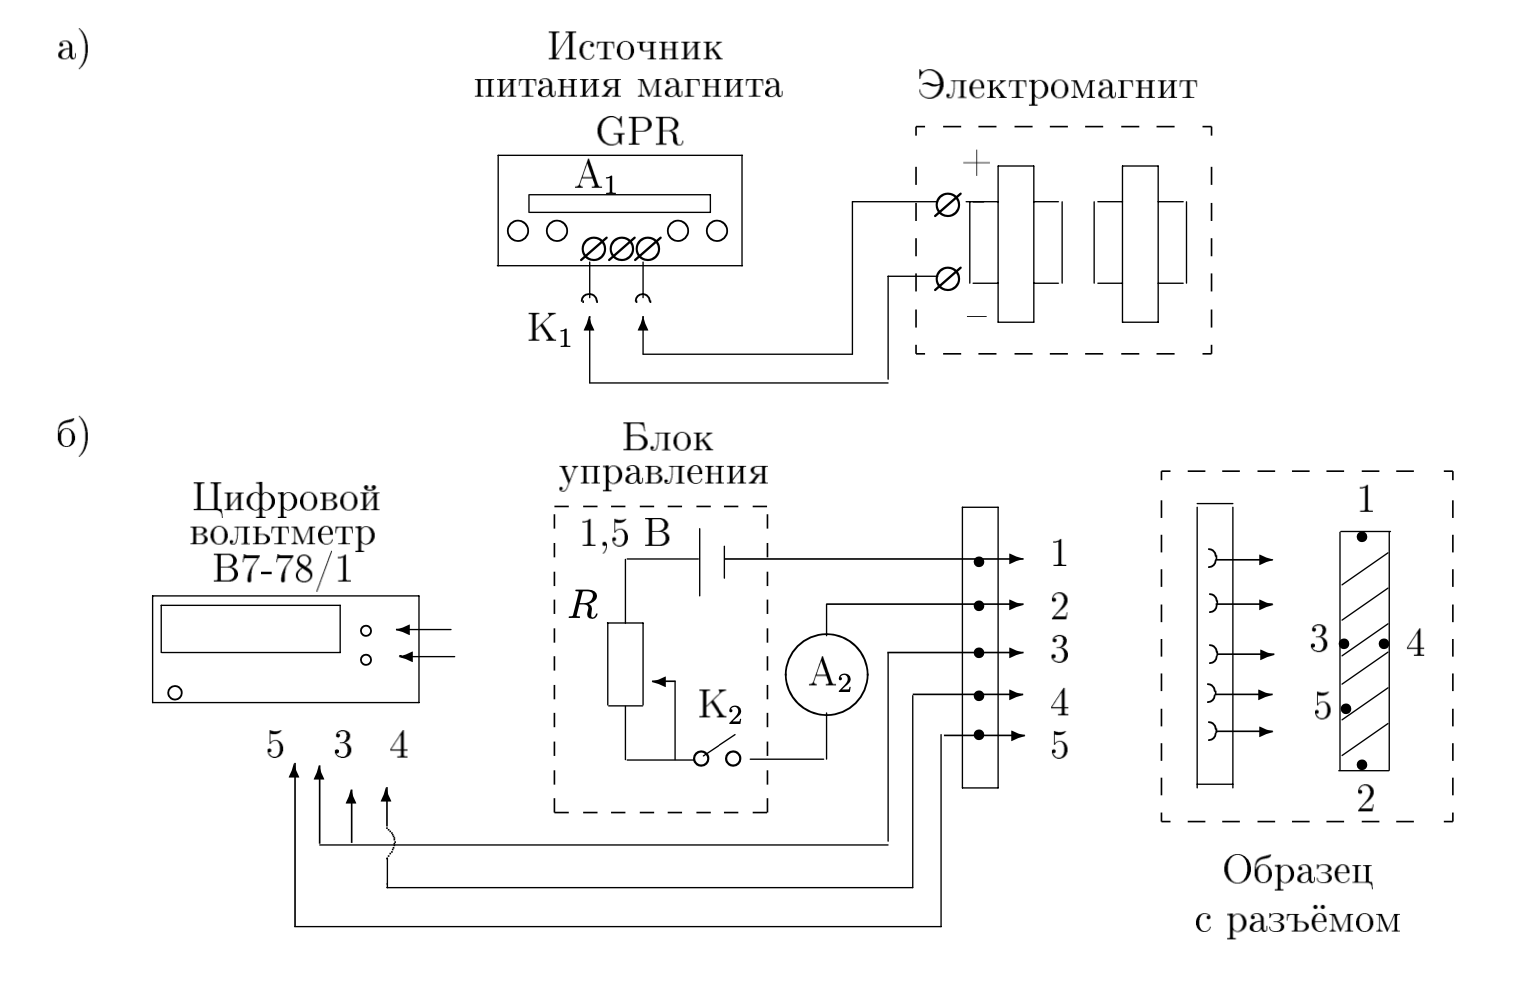
\includegraphics[width=\linewidth]{scheme.png}
    \caption{Cхема установки для исследования эффекта Холла в полупроводниках}
\end{figure}

В зазоре электромагнита создаётся постоянное магнитное поле, величину которого можно менять регуляторами источника питания электромагнита. Градуировка магнита проводится при помощи милливеберметра.\\
Образец из легированного германия, смонтированный в специальном держателе, подключается к источнику питания. При замыкании К$_2$ вдоль длинной стороны образца течёт ток, величина которого регулируется реостатом $R$ и измеряется миллиамперметром. В образце, помещённом в зазор, возникает разность потенциалов $U_{34}$, которая измеряется с помощью цифрового вольтметра.\\
Влияние омического падения напряжения исключается измерением напряжения $U_0$ между 3 и 4 в отсутствие магнитного поля. По знаку $\mathcal{E} = U_{34} \pm U_0$ можно определить характер проводимости -- электронный или дырочный, зная напрявление тока в образце и напрвление магнитного поля.\\
Померив ток $I_{35}$ в образце и напряжение $U_{35}$ между контактами 3 и 5 в отсутствие магнитного поля можно рассчитать проводимость материала по формуле
$$
\sigma = \frac{I \ L_{35}}{U_{35}a\ l},
$$
где $L_{35}$ -- расстояние между контактами 3 и 5, а $a$ и $l$ -- толщина и ширина образца.

\subsection*{Результаты измерений и обработка данных}
При помощи датчика установим зависимость магнитной индукции $B$ от силы тока $I_M$, постепенно уменьшая ее от максимума до минимума.
При измерении индукции имеет значение также ориентация датчика, в связи с чем показания следует снимать в обоих положениях, далее усредняя полученные значения. 
Результаты занесем в таблицу 1.

\begin{table}[htp]
    \centering
    \begin{tabular}[]{|c|c|c|c|c|c|c|c|c|c|c|c|c|}
        \hline
        $I_M$, А  & \multicolumn{2}{|c|}{1.07} & \multicolumn{2}{|c|}{0.89}  & \multicolumn{2}{|c|}{0.70}  & \multicolumn{2}{|c|}{0.53}  & \multicolumn{2}{|c|}{0.36}  & \multicolumn{2}{|c|}{0.18} \\
        \hline
        $B$, мТл &  946 & 980 & 850 & 878 & 746 & 715 & 550 & 582 & 399 & 367 & 190 & 220\\
        \hline
    \end{tabular}
    \caption{Зависимость магнитной индукции от тока}
\end{table}

Построим график по полученным данным (рис. 2)
\begin{figure}[htp]
    \centering
    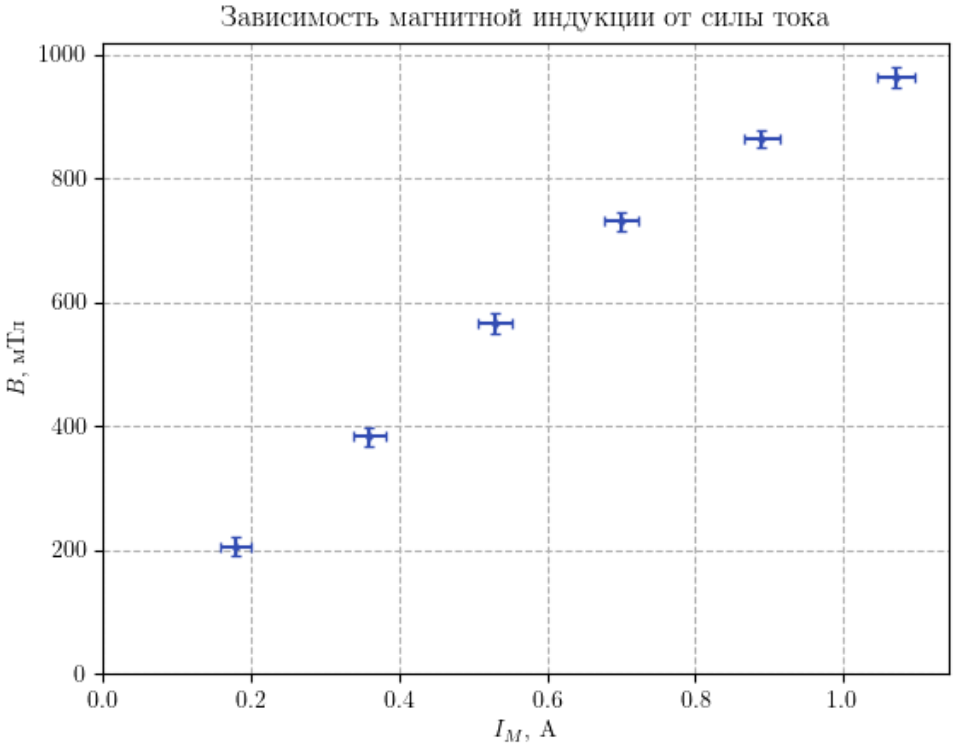
\includegraphics[width=0.72\linewidth]{B_I.png}
    \caption{Зависимость магнитной индукции от тока}
\end{figure}

Коэффицент наклона прямой по МНК равен $k_1 = 970 \pm 30 {мТл\over А}$.

Теперь вставим исследуемый образец между полюсами магнита и установим зависимость напряжения $U_{34}$ от силы тока $I_M$ через электромагнит.
Измерения проведем при тех же значениях тока, что были установлены в предыдущем опыте.
Значения тока через образец будем изменять в пределах от 30 мА до 100 мА.

Также начальное напряжение $U_0$, отображающееся на вольтметре при отсутствии образца между полюсами, следует принять за нулевое.

Измерения при максимальном токе через образец проведем для обоих направлений поля через него, развернув образец.

\begin{table}[htp]
    \centering
    \begin{tabular}[]{|c|c|c|c|c|c|c|c|}
        \hline
        $I$, мА & $U_{0}$, мкВ & \multicolumn{6}{|c|}{$U_{34}$, мкВ} \\
        \hline
        30 & -56 & 55 & 45 & 31& 14& 5& -30 \\
        \hline
        40 & -74 & 73 & 59& 41 & 17 & -8& -39 \\
        \hline
        50 & -93 & 92 & 75 & 52 & 22 & -10 & -49 \\
        \hline
        60 & -111 & 108 & 91 & 62 & 28 & -11 & -60\\
        \hline
        70 & -131 & 125 & 106 & 72 & 32 & -16 & -68  \\
        \hline 
        80 & -149 & 144 & 122 & 82& 38 & -15& -79 \\
        \hline
        90 & -168 & 162 & 136 & 92 &42 & -19& -90 \\
        \hline
        100 & -186& 179 & 149 & 104& 46& -19 & -99 \\
        \hline
        100 $\downarrow$ & -186& -571 & -540 & -487 & -427 & -355 & -273  \\
        \hline
    \end{tabular}
    \caption{Зависимость напряжения от тока}
\end{table}
\begin{figure*}[h!]
    \begin{flushright}
        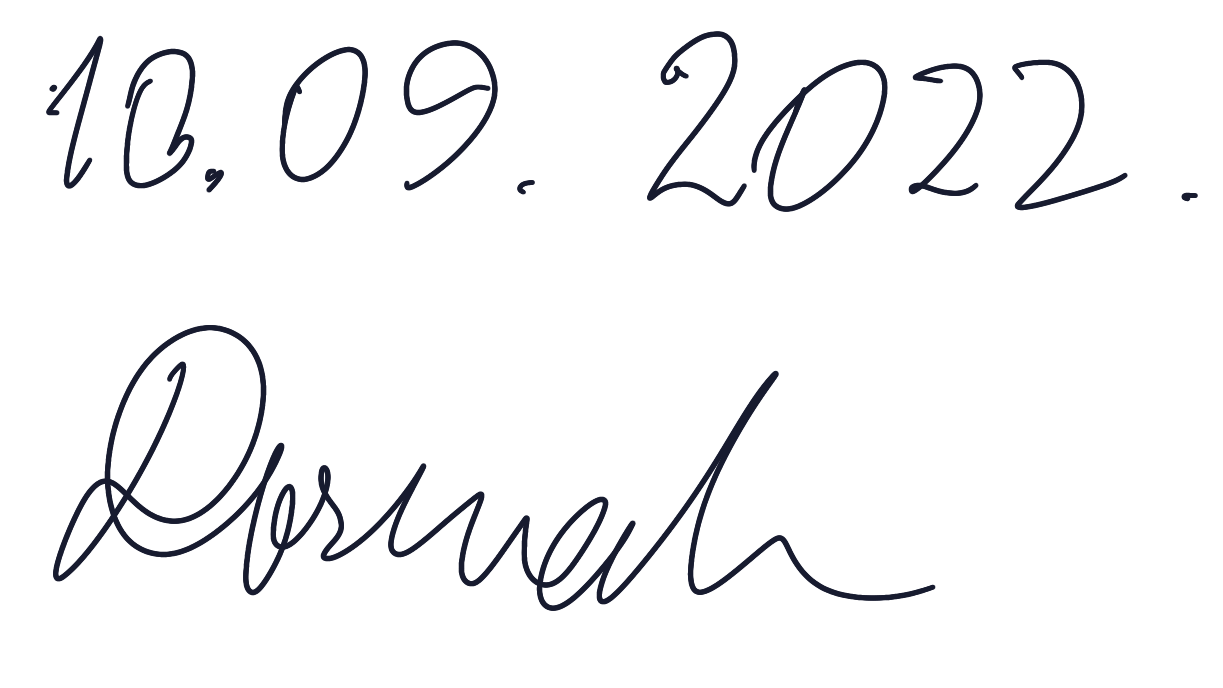
\includegraphics[scale=0.17]{signa.png}
    \end{flushright}
\end{figure*}

Отобразим зависимость ЭДС Холла от тока (рис. 4)
\begin{figure}[h!]
    \centering
    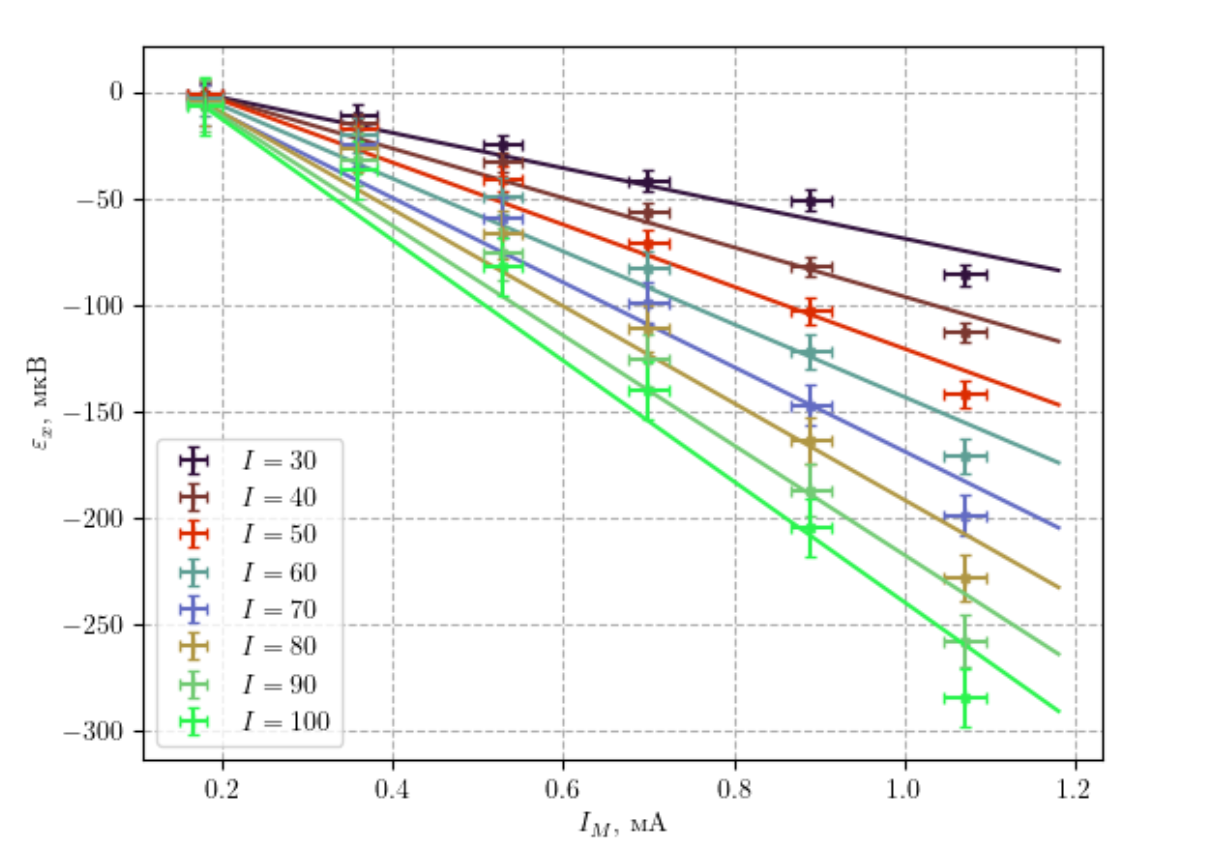
\includegraphics[width=0.7\linewidth]{e(im).png}
    \caption{Зависимость ЭДС Холла от тока}
\end{figure}

\newpage
Теперь найдем зависимость угла наклона от $I$.

\begin{table}[h]
    \centering
    \begin{tabular}[]{|c|c|c|c|c|c|c|c|c|}
        \hline
        $I$, мА &30 &40&50&60&70&80&90&100\\
        \hline
        $k$, ${мВ \over А}$, & -82.9 & -116.2 & -146.0 & -171.2 & -198.8 & -227.8 & -258.1 & -283.9 \\
        \hline
        $\sigma_k$, ${мВ \over А}$ & 5.0 & 4.6 & 6.0 & 8.3 & 9.5 & 11.0 & 12.2 & 13.6 \\
        \hline
    \end{tabular}
\end{table}

\begin{figure}[h!]
    \centering
    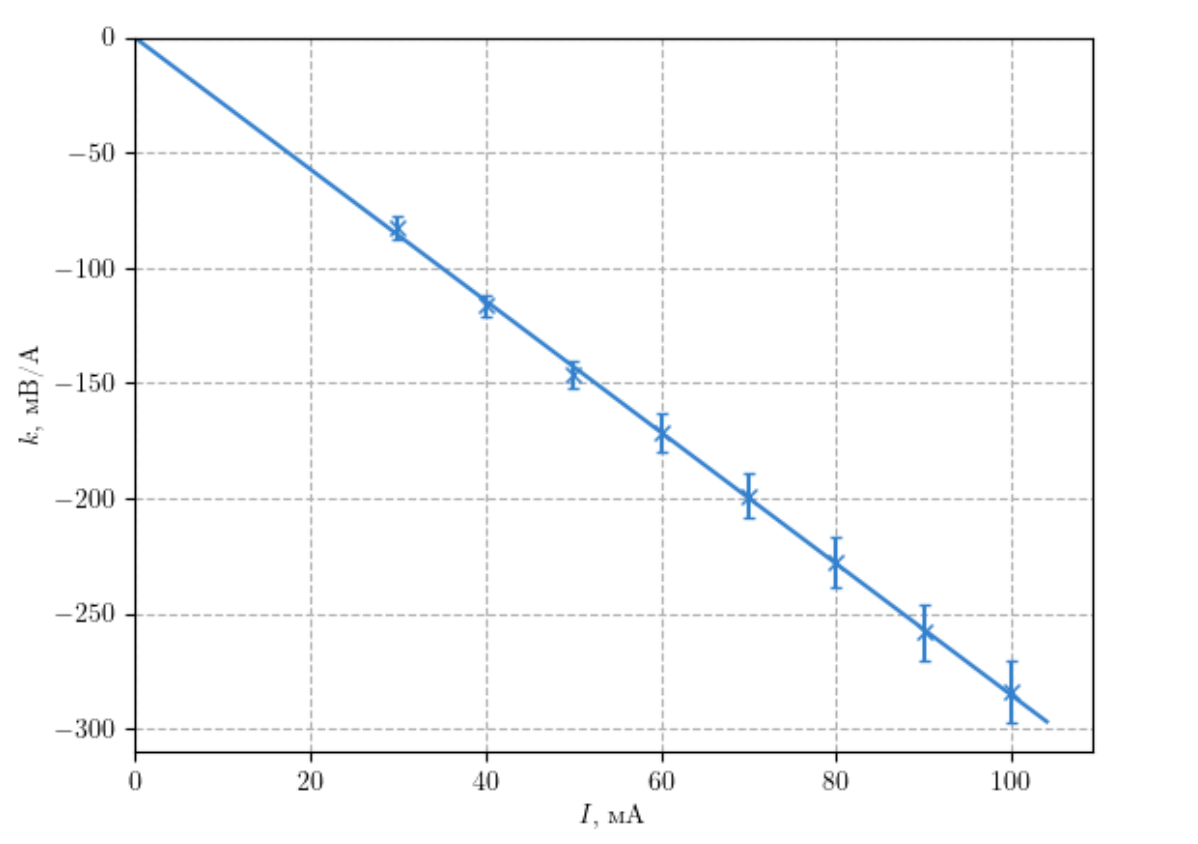
\includegraphics[width=0.7\linewidth]{k(I).png}
    \caption{Зависимость $k(I)$}
\end{figure}

Коэффицент наклона $k_2 = -2.85 \pm 0.01 {В \over А^2}$. 

Также указанные на образце параметры: $a$ = 2.2 мм, $L$ = 6.0 мм, $l$ =7 мм.

\begin{equation*}
    R_x = -{\varepsilon_x \over IB}a = -{\varepsilon_x\over I \cdot I_M} {I_M \over B}a = -{k_2 \over k_1} a = (750 \pm 50) \cdot 10^{-3}{В\cdot м \over Тл\cdot А}
\end{equation*}

Концентрация носителей заряда $n = {1 \over e R_x} = (8.3 \pm 0.6) \cdot 10^{18} {1\over м^3}$

Для определения удельной проводимости выключим источник питания и измерим падение напряжения $U_{35}$ (1 мА)= -2,488 мВ. 
Тогда $\sigma = {IL \over U_{35}al} = 156.6 \pm 3 {1 \over Ом \cdot м}$.
Также вычислим подвижность носителей заряда $b = {\sigma \over en} = \sigma R_x = (0.12 \pm 0.01) \cdot 10^{-3} {м^2 \over В \cdot с}$

\subsection*{Подведение итогов}
В ходе работы изучено явление Холла на основе образца. 
Также вычислена постоянная Холла для исследуемого образца $R_x = (750 \pm 50) \cdot 10^{-6}{В\cdot м \over Тл\cdot А}\ (\varepsilon \approx 7 \%)$, концентрация носителей заряда $n = (8.3 \pm 0.6) \cdot 10^{21} {1\over м^3}\ (\varepsilon \approx 8\%)$, 
удельная проводимость $\sigma = 156.6 \pm 3 {1 \over Ом \cdot м}\ (\varepsilon \approx 2\%)$ и подвижность носителей заряда $b = 120 \pm 10 {cм^2 \over В \cdot с}\ (\varepsilon \approx 9\%)$. 
Полученные данные могут отличаться от табличных в связи с сильной чувствительностью используемого прибора к нагреву, происходящему при проходе через него тока, и большим количеством примесей в рассматриваемом образце.
\end{document}